\documentclass{article}
\usepackage[margin=1.25in]{geometry}
\usepackage{amsmath, amssymb, setspace, enumerate, enumitem}
\usepackage{tikz}
\usetikzlibrary{automata, positioning, arrows}
\tikzset{
->, % makes the edges directed
>=stealth', % makes the arrow heads bold
node distance=3cm, % specifies the minimum distance between two nodes. Change if necessary.
every state/.style={thick, fill=gray!10}, % sets the properties for each ’state’ node
}
\usepackage{graphicx}
\onehalfspacing

\begin{document}
    \noindent \textbf{*Problem 13.42: To determine if a graph G with 50 vertices is 3-colorable, you test all possible 3-colorings. Your computer checks a million 3-colorings per second. Estimate how long it is going to take, in the worst case.}
    \\ Test all 50 vertices with 3 colors:
    \\ By sum and product law, we know that the number of subsequent choices aren't affected by the previous, we can conclude that each vertices will have 3 possible choices. All possible 3-colorings are calculated by $3^{50}$
    \\ Given that the computer checks a million 3-colorings per second, we can calculate:
    \begin{align*}
        T &= \frac{3^{50}}{10^7}\\
        & \approx 7.179 \times 10^{16}
    \end{align*}
    \noindent This means that all possible 3 colorings can be calculated in about {\LARGE $\boxed{\mathbf{7.179 \times 10^{16}}}$} seconds.
    
    \noindent\\[0.25in]
    \noindent \textbf{*Problem 13.50. How many 7-digit phone-numbers are non-decreasing (each digit is not less than the previous one.)}
    \\ For this problems, we can think of it as choosing 7 random number out of a bucket, each number is placed 7 times, so there is a possible of a single number being chosen
    7 times. We can think of it as this 10 containers and we have 7 items to place in 10 different containers. Since we have 10 different containers for the 7 items, we can select 
    k = 7 numbers from r = 10 containers. With this, we can derive the k-subset formula with repetition equal to ${10 + 7 - 1 \choose 10 - 1}$ = {\LARGE $\boxed{\mathbf{16 \choose 9}}$}
    \noindent\\[0.25in]
    \noindent \textbf{*Problem 14.15(b-c). Consider the binary strings consisting of 10 bits.}
    \begin{enumerate}[label=(\alph*)]
        \item \textbf{How many contain (i) 5 or more consecutive 1’s (ii) 5 or more consecutive 0’s?}
        \begin{enumerate}[label=(\roman*)]
            \item 5 or more consecutive 1's
            \\ For a string of 5 bits, we have 6 possible start locations to begin placing 1's to make 
            sure that we reach 5 consecutive 1's. For the remaining 5 numbers, we have 2 options, represented
            by:
            \begin{verbatim}
                { {1, 1, 1, 1, 1}, x, x, x, x, x}
                x = dont care
            \end{verbatim}
            There are $6 \times 2^5$ choices for this subset. A double counting issue such as this arises:
            \begin{verbatim}
                { x {1, 1, 1, 1, 1}, x, x, x, x}
            \end{verbatim}
            where this subset can produce the same string as the one above.\\
            Given that there are 5 different "dont cares", we can restrict each of them, leaving the other 4 free to have all the repeated, forming the equation $2^4 \times 5$\\
            Removing them from our original subset, we get $6 \times 2^5 - 5 \times 2^4$ = {\LARGE $\boxed{\mathbf{112}}$}
            \item 5 or more consecutive 0's
            \\ following the same logic, we can deduct this is the same, at {\LARGE $\boxed{\mathbf{112}}$}
            possible binary strings.
        \end{enumerate}
        \item \textbf{How many contain 5 or more consecutive 0’s or 5 or more consecutive 1’s?}
        For every binary string that have 5 or more consecutive 1's, just replace those with 0's
        to achieve $2 \times 112$ possibilities. There are two possibilities that are double
        counted: 1111100000 and 0000011111 = {\LARGE $\boxed{\mathbf{2 \times 112 - 2}}$}
    \end{enumerate}

    \noindent\\[0.25in]
    \noindent \textbf{*Problem 14.34. Consider all permutations of \{1, 2, 3, 4, 5, 6\}. A permutation is good if any of the sub-sequences 12, 23, or 56 appear. How many good permutations are there?}
    \\ Let us create subsets like such:
    \begin{verbatim}
        1. {{1, 2}, 3, 4, 5, 6} subsequence 1,2 appear
        2. {1, {2, 3}, 4, 5, 6} subsequence 2,3 appear
        3. {1, 2, 3, 4, {5, 6}} subsequence 5,6 appear
        4. {{1, 2, 3}, 4, 5, 6} subsequence 1,2 and 2,3 appear
        5. {{1, 2}, 3, 4, {5, 6}} subsequence 1,2 and 5,6 appear
        6. {1, {2, 3}, 4, {5, 6}} subsequence 2,3 and 5,6 appear
        7. {{1, 2, 3}, 4, {5, 6}} all subsequence appear
    \end{verbatim}
    \begin{enumerate}[label=1-3: ]
        \item Total number of subsequences that appears, with duplicated = $3 \times 5!$
    \end{enumerate}
    \begin{enumerate}[label=4-6: ]
        \item Number that 2 sequences appear = $4!$, total of $3 \times 4!$
    \end{enumerate}
    \begin{enumerate}[label=7: ]
        \item Number that all sequences appear = $3!$
    \end{enumerate}
    We can get rid of subset 4-6 by subtracting, but for subset 7, since all sequences appear, we removed it before so we have to add it back.
    \begin{align*}
        3 \times 5! - 3 \times 4! + 3! = 294
    \end{align*}
    There are {\LARGE $\boxed{\mathbf{294}}$} possible permutations that contains 12, 23, or 56.

    \noindent\\[0.25in]
    \noindent\textbf{*Problem 14.63(g). Here are some counting problems on graphs to challenge you.}
    \begin{enumerate}[label=(g)]
        \item \textbf{How many Hamiltonian cycles are in $K_{n,n}$? [Hint: a Hamiltonian cycle is a cycle on
        graph $G = (V, E)$ that starts and ends at vertex $v_0\;\epsilon\;V$ , visiting each vertex in set
        $V-\{v_0\}$ (i.e., all other vertices) exactly once.]}
        \\ There are n vertices on each side. If I start from the left side, I can choose $n$ vertices on the right side.
        After choosing from the right side, I have $n-1$ vertices to choose from the left side, and so on. If I have n = 4, the
        possibilities sequence will go from \{4, 3, 3, 2, 2, 1, 1, 1\}, starting from any vertex. Each vertex has $n \times ((n-1)!)^2$
        possibility of hamiltonian cycles. For a bipartite graph $K_{n,n}$, there are $2n$ total vertices. There is a total of {\LARGE $\boxed{\mathbf{2n(n\times((n-1)!)^2)}}$} possibilities.
    \end{enumerate}

    \noindent\\[0.25in]
    \noindent\textbf{*Problem 15.12. Roll a 6-sided die 5 times. What is the probability: (a) some number repeats (b) you get no sixes?}
    \begin{enumerate}[label=(\alph*)]
        \item some number repeats
        \\ Total number of combinations when rolling a die 5 times = $6^5$
        \\ For a number not to repeat, for each roll, the number of possibilities after is one less. To achieve 5 rolls without any repeated the numbers, the product would be $6 \times 5 \times 4 \times 3 \times 2$, or $6!$.
        \\ To solve this, we can remove the total number of rows without a repeated number from the total combinations, leaving us with $6^5 - 6!$. To get the probability, we can divide it by the total:
        \begin{align*}
            \frac{6^5 - 6!}{6^5} = 0.907
        \end{align*}
        Probabilities of rolling a 6 sided die 5 times and some number repeats = {\LARGE $\boxed{\mathbf{90.7\%}}$}
        % \\ A die is rolled 5 times, for a number to repeat, you need two rolls to be the same number, we can choose any of the 6 numbers to be that number that repeats = $(1\times1)\times6$
        % \\ For the rest of the 3 numbers, we have 6 possibilities of what they can be = $6^3$
        % \\ Multiplied together, we get $(1\times1)\times6\times6^3$ = $6^4$. Considering that they don't have to be consecutive, the second roll can be in any of the 4 other spots. To achieve this, multiply by 4 = $6^4 \times 4$
        
        \item no sixes
        \\ Total number of combinations stay the same at $6^5$
        \\ 6 is eliminated, only 5 possible numbers are left to choose from = $5^5$
        \\ Probabilities of rolling a 6 sided die 5 times and having no 6's = {\large $\frac{5^5}{6^5}$} or {\LARGE $\boxed{\mathbf{40.2\%}}$}
    \end{enumerate}

    \noindent\\[0.25in]
    \noindent\textbf{*Problem 24.11(f,h,w). Give DFAs for the following languages, a.k.a., computing problems.}
    \begin{enumerate}[label=(\alph*)]
        \setcounter{enumi}{5}
        \item $\mathbf{\mathcal{L}=\{1^{\bullet 2n}01^{\bullet 2k+1}\ |\ n,k\ge 0\}}$.
        \setcounter{enumi}{7}
        \begin{center}
            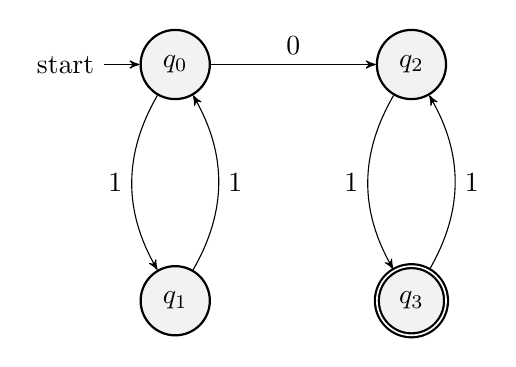
\begin{tikzpicture}
                \node[state, initial] (q0) {$q_0$};
                \node[state, below of=q0] (q1) {$q_1$};
                \node[state, right of=q0] (q2) {$q_2$};
                \node[state, below of=q2, accepting] (q3) {$q_3$};
                \draw (q0) edge[above] node{0} (q2);
                \draw (q0) edge[below, bend right, left=0.3] node{1} (q1);
                \draw (q1) edge[above, bend right, right=0.3] node{1} (q0);
                \draw (q2) edge[below, bend right, left=0.3] node{1} (q3);
                \draw (q3) edge[above, bend right, right=0.3] node{1} (q2);
            \end{tikzpicture}
        \end{center}
        \item \textbf{Strings which begin with 10 and end with 01.}
        \setcounter{enumi}{22}
        \begin{center}
            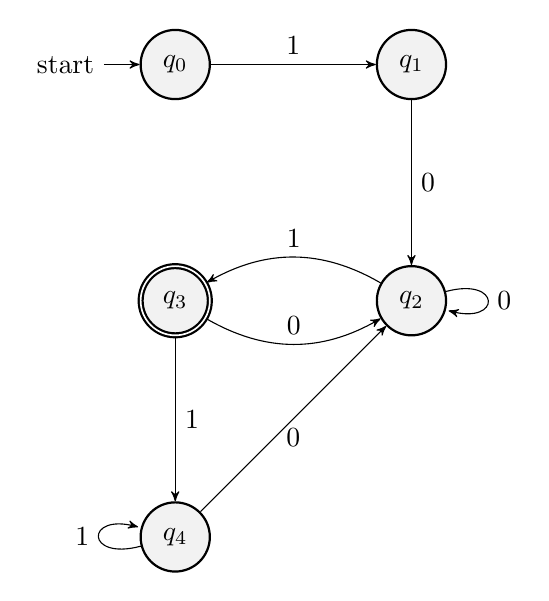
\begin{tikzpicture}
                \node[state, initial] (q0) {$q_0$};
                \node[state, right of=q0] (q1) {$q_1$};
                \node[state, below of=q1] (q2) {$q_2$};
                \node[state, left of=q2, accepting] (q3) {$q_3$};
                \node[state, below of=q3] (q4) {$q_4$};

                \draw (q0) edge[above] node{1} (q1);
                \draw (q1) edge[right] node{0} (q2);
                \draw (q2) edge[loop right] node{0} (q2);
                \draw (q2) edge[above, bend right] node{1} (q3);
                \draw (q3) edge[right] node{1} (q4);
                \draw (q4) edge[loop left] node{1} (q4);
                \draw (q4) edge[below] node{0} (q2);
                \draw (q3) edge[above, bend right] node{0} (q2);
            \end{tikzpicture}
        \end{center}
        \item \textbf{Strings whose length is divisible by 3.}
        \begin{center}
            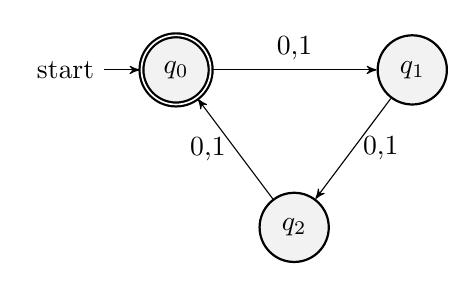
\begin{tikzpicture}
                \node[state, initial, accepting] (q0) {$q_0$};
                \node[state, right of=q0] (q1) {$q_1$};
                \node[state] at (1.5, -2) (q2) {$q_2$};

                \draw (q0) edge[above] node{0,1} (q1);
                \draw (q1) edge[right] node{0,1} (q2);
                \draw (q2) edge[left] node{0,1} (q0);
            \end{tikzpicture}
        \end{center}
    \end{enumerate}

    \noindent\\[0.25in]
    \noindent\textbf{*Problem 25.7 Give a DFA and a CFG for each problem.}
    \begin{enumerate}[label=(\alph*)]
        \item $\mathbf{\mathcal{L}=\{01^{\bullet n}\ |\ n\ge 0\}}$
        \begin{center}
            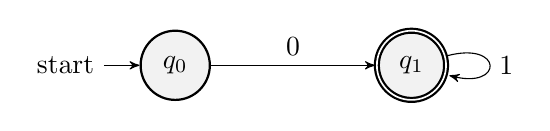
\begin{tikzpicture}
                \node[state, initial] (q0) {$q_0$};
                \node[state, right of=q0, accepting] (q1) {$q_1$};

                \draw (q0) edge[above] node{0} (q1);
                \draw (q1) edge[loop right] node{1} (q1);
            \end{tikzpicture}

            \begin{tabular}{l l}
                $S \rightarrow$ & $0$ $|$ $ST_1$\\
                $T_1 \rightarrow$ & $1$
            \end{tabular}
        \end{center}
        \item $\mathbf{\mathcal{L}=\{0^{\bullet n}1^{\bullet n}\ |\ 0\le n\le 5\}}$
        \begin{center}
            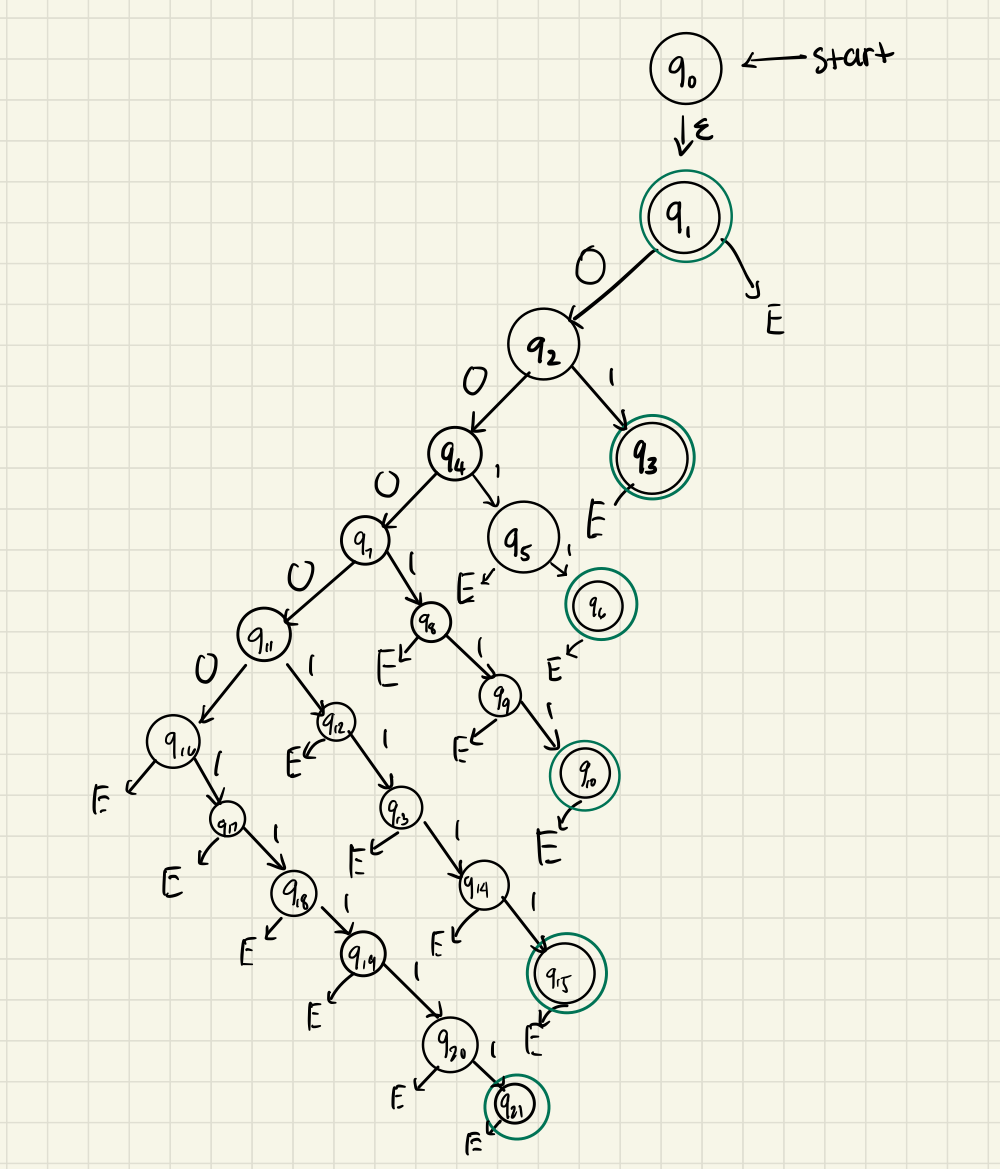
\includegraphics[scale=0.5]{p25_7b.jpg}

            \begin{tabular}{l l}
                $S \rightarrow$ & $\epsilon$ $|$ $01$ $|$ $0011$ $|$ $000111$ $|$ $00001111$ $|$ $0000011111$\\
            \end{tabular}
        \end{center}
        \item $\mathbf{\mathcal{L}=\{}$ \textbf{strings which end in a 1} $\mathbf{\}}$
        \begin{center}
            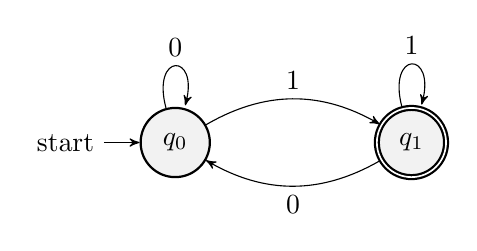
\begin{tikzpicture}
                \node[state, initial] (q0) {$q_0$};
                \node[state, right of=q0, accepting] (q1) {$q_1$};

                \draw (q0) edge[loop above] node{0} (q0);
                \draw (q0) edge[above, bend left] node{1} (q1);
                \draw (q1) edge[below, bend left] node{0} (q0);
                \draw (q1) edge[loop above] node{1} (q1);
            \end{tikzpicture}

            \begin{tabular}{l l}
                $S \rightarrow$ & $1$ $|$ $T_0S$ $|$ $T_1S$\\
                $T_0 \rightarrow$ & $0$ \\
                $T_1 \rightarrow$ & $1$
            \end{tabular}
        \end{center}
    \end{enumerate}

\end{document}